% \wenfei{edit until here}
\section{Evaluation}
\vspace{-0.05in}
\subsection{Best GOP}
The previous section indicates that reducing the keyframe interval may cut down the frame dropping. Therefore in this section, we evaluate the method: reducing keyframe interval.
\textbf{Implementation and experiment setup.}
We control the outbound throughput of broadcaster to a constant level, and introduce a 2-second interruption. We record the number of frame drops as metrics to evaluate these methods. The frame rate in this paper usually sets as 30.

\begin{figure}[htb]
\centering
\begin{subfigure}[b]{.8\columnwidth}
\centering
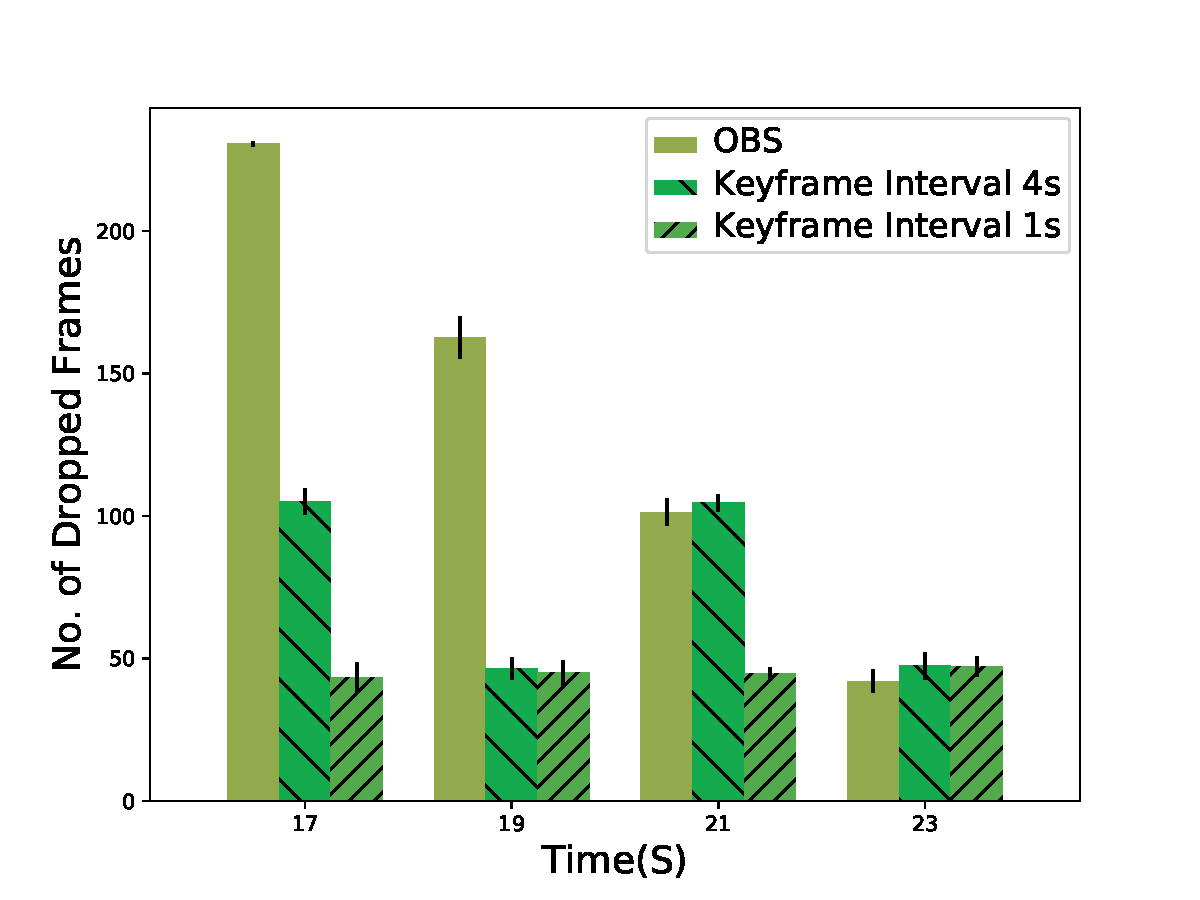
\includegraphics[width=\textwidth]{fig/eval_IframeInterval_drop.pdf}
\caption{Frame drop with varying I frame interval}
\label{fig:iframe-drop}\mylabel{fig:iframe-drop}
\end{subfigure}

\iffalse
\minipage{0.32\textwidth}
  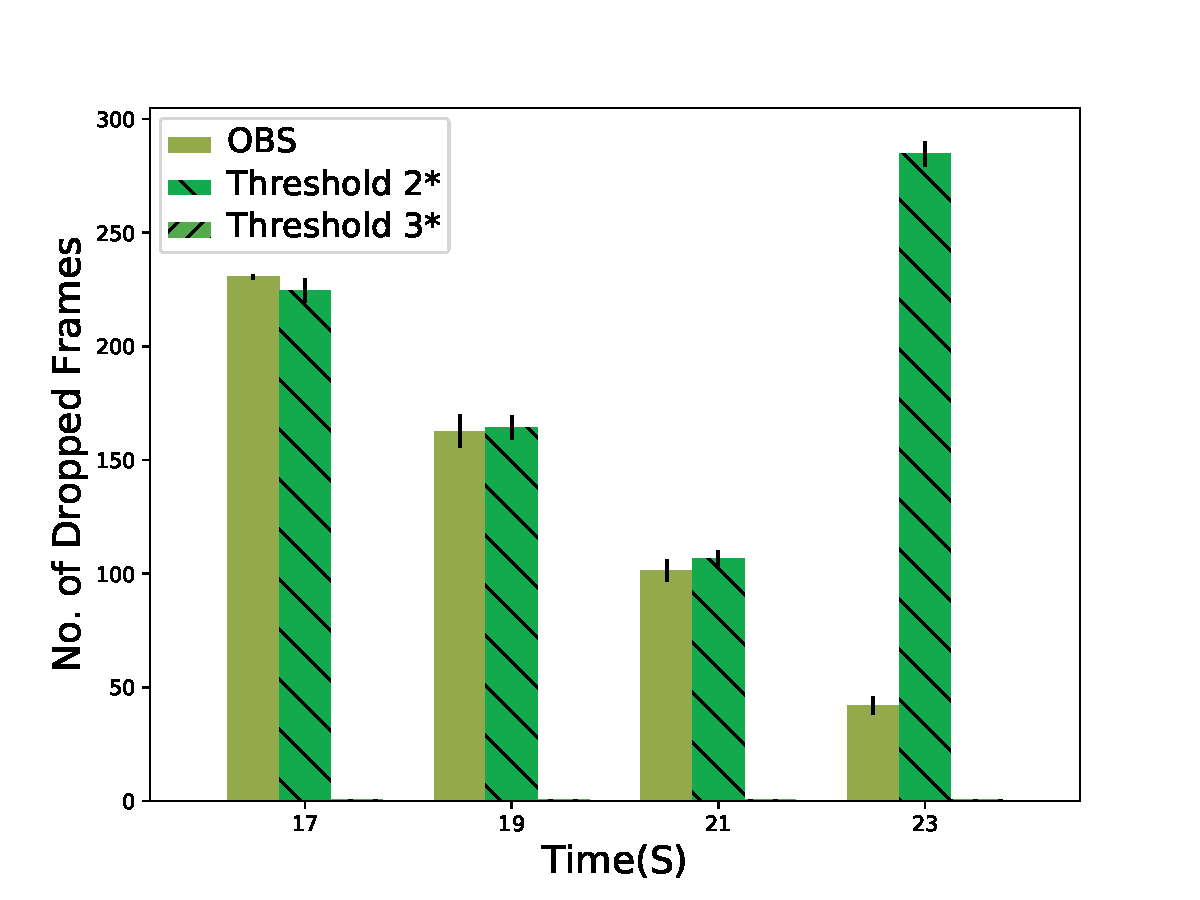
\includegraphics[width=\linewidth]{fig/eval_threshold_drop.pdf}
  \caption{Frame drop with varying threshold}
  \label{fig:threshold-drop}\mylabel{fig:threshold-drop}
\endminipage\hfill
\minipage{0.32\textwidth}
  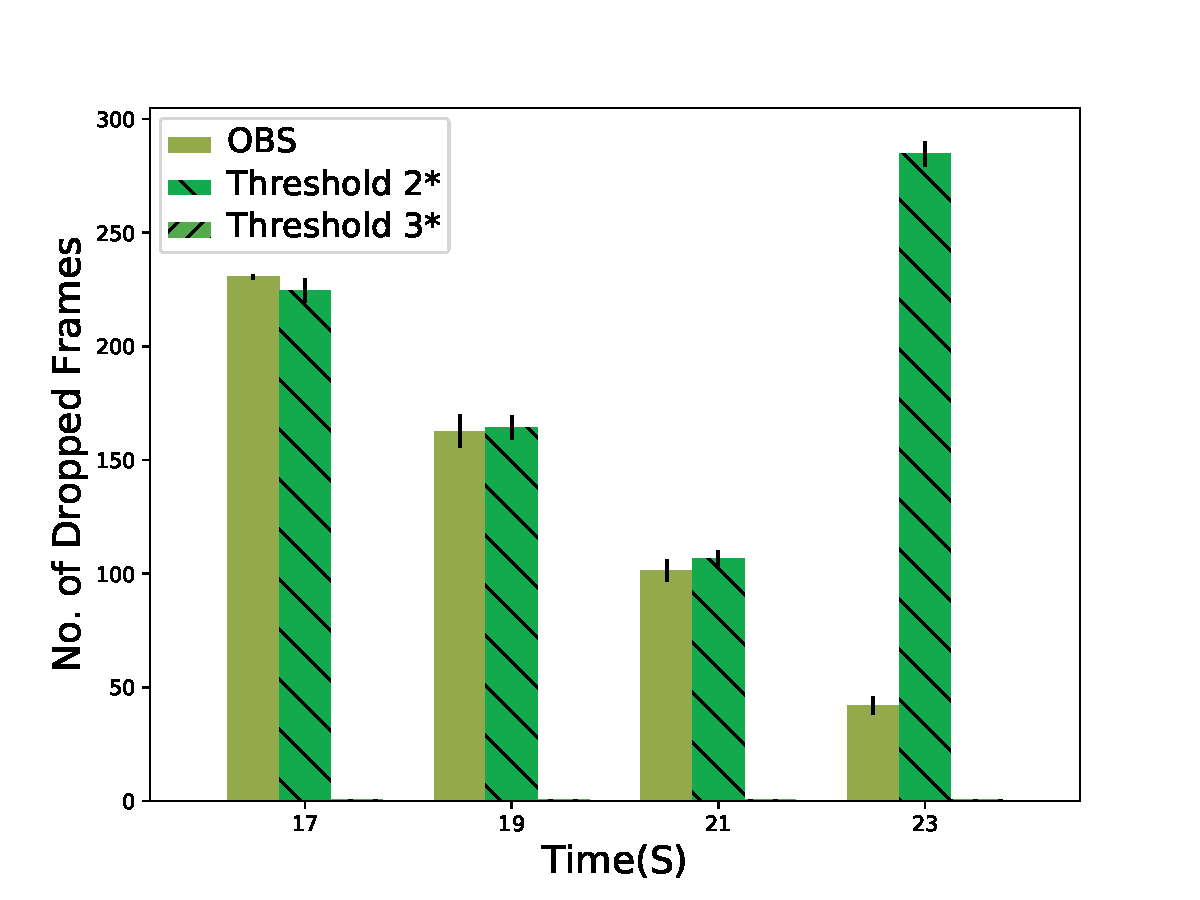
\includegraphics[width=\linewidth]{fig/eval_threshold_drop.pdf}
  \caption{Timeliness with varying I frame interval}
  \label{fig:iframe-timeliness}\mylabel{fig:iframe-timeliness}
\endminipage
\fi

\end{figure}

\iffalse
\begin{figure}
\centering
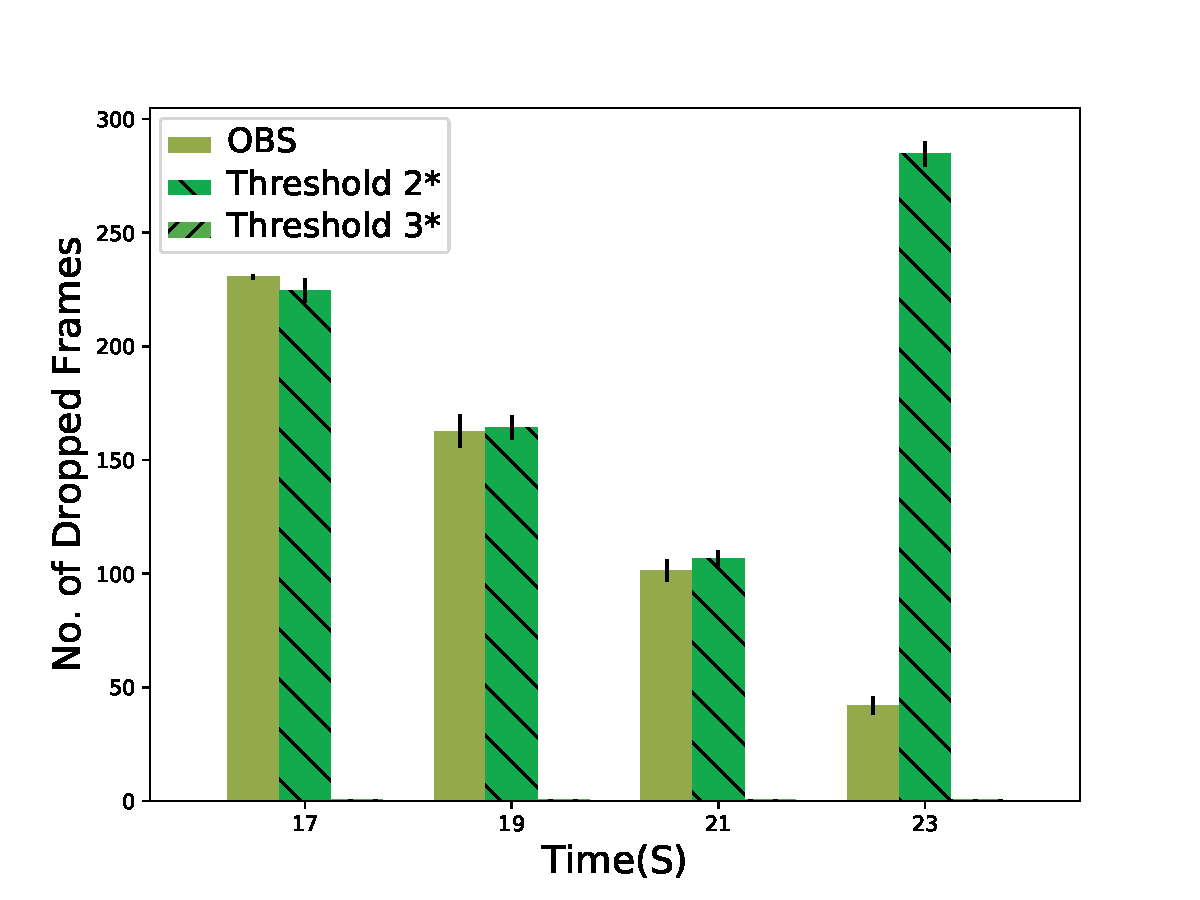
\includegraphics[width=0.32\textwidth]{fig/eval_threshold_drop.pdf}
\caption{Timeliness with varying threshold}
\label{fig:threshold-timeliness}\mylabel{fig:threshold-timeliness}
\end{figure}
\fi 
\textbf{Varying keyframe interval.} The default I frame interval of OBS is 8 seconds, and we adjust it to 4s and 1s in experiments. The frame drops are shown in Figure~\ref{fig:iframe-drop}. We can observe that in each individual experiment, when the interruption starts earlier in a GOP, more frames are dropped. Because an early frame has more following frames depending on it. For default setting, 8 second keyframe interval, when interruption starts at 17s, 19s, 21s, and 23s, the number of frame drops is 238, 164, 105, and 48.
\iffalse
Also, the number of frame drop appears to have the same period with the keyframe interval (e.g., when keyframe interval is 4s, the number of frame drops is 102, 47, 103, and 48 when interruption starts at 17s, 19s, 21s, and 23s, demonstrating a period of 4s.).
\fi
Comparing bars within the group of 17s, we find that smaller keyframe interval significantly reduces the number of frame drop (i.e., from 238, to 102, and 46 when the interval is from 8s to 4s and 1s). However, this reduction is not significant for the group of 23s, because 23s is near the end of a GOP in all cases (8s, 4s, and 1s interval), and there are less frames depending on the frame at 23s.

This experiment shows that if we can eliminate the dependency between frames, an occasional network jitter would only affect frames within a limited duration near the jitter, instead of cascadingly affecting frames in following several seconds.

Reducing keyframe interval is an intractable issue because that adjusting would cause video quality degradation.

\textbf{Video quality and GOP} As mentioned above, the size of GOP needs a tradeoff between video quality and frame dropping. To guide the choice of keyframe interval, we try to vary the GOP and encode many uncompressed streaming using the x264 encoder \cite{x264}. A truth is that the x264 encoder use the delta intermode coding. Thus a larger GOP is much more likely to introduce the accumulative errors, and GOP is recommended smaller than 250 frames. Nevertheless how to determine the specific value is still sophisticated. The video dataset we use contains SD content, HD content, gaming, and 4k content in variety \cite{video_dataset}. The relationship between normalized SSIM and GOP size is displayed in Fig~\ref{fig:ssim_gop}.
We pick four from many videos to represent the result. From the figure, we can see when the GOP size is larger than 0.5s, the SSIM keeps almost the same, with few changes. Additionally combining the previous two experiments, a GOP size larger than 0.5s can achieve better video quality; and a smaller GOP size will reduce the frame dropping. We can see that GOP size between $[0.5,2]$s is probably the best choice for keyframe interval.

\iffalse
\begin{table}[htb]
\centering
\caption{No. of Dropped Frames}
\label{tab:bitrate}\mylabel{tab:bitrate}

\begin{tabular}{|l|l|l|l|l|}
\hline
Bitrate(kbps)          & 1000  & 1500  & 2000  & 2500  \\ \hline
Average Dropped Frames & 148.2 & 148.2 & 149.0 & 150.6 \\ \hline
\end{tabular}
\end{table}
\textbf{Varying bitrate.}
To make the conclusion more visible, we fix keyframe interval to be 8s and introduce network interruption between 19s and 21s. In different experiments, we provide sufficient network bandwidth and vary the bitrate to be 1000kbps, 1500kbps, 2000kbps, and 2500kbps. The frame drop is shown in Table~\ref{tab:bitrate}. The different bitrates do not make much difference, the number of drop in all cases is about 149.

\textbf{Summary.} We summarize and get conclusions. First, reducing keyframe interval leads to less frame drop. Second, bitrate does not influence frame drop for the short-term case, but the quality of each picture. Preliminary Evaluation points out that a small GOP is one useful try.
\fi

\vspace{-0.05in}
\subsection{Greedy Drop Strategy}
To measure the performance, we compare the performance with two algorithms, there are namely Oracle, GreedyDrop(Algorithm~\ref{alg:greedy-drop}). Oracle, the offline optimal solution by the brute-force search, which has an exponential time complexity. We pick out one part from the dataset, and the trace lasts for $30$ seconds. During the period both bandwidth fading and bandwidth fluctuating appears. The frame rate is $30$ fps, and the total number of frame equals $900$.

\begin{table}[tb]
\centering
\caption{The Reduction of Frame Drops Normalized to Default OBS}
\label{tab_drop}
{\setlength{\tabcolsep}{1pt}
\begin{tabular}{|c|c|l|}
\hline
\textbf{Algorithm} &\textbf{Play Failure(s)} & \textbf{Percentage}    \\ \hline
Oracle    &265    &$80\%$           \\ \hline
GreedyDrop  &274  &$85.6\%$              \\ \hline
\end{tabular}}
\vspace{-0.1in}
\end{table}

\begin{figure}[htb]
\centering
\begin{subfigure}[b]{.45\columnwidth}
\centering
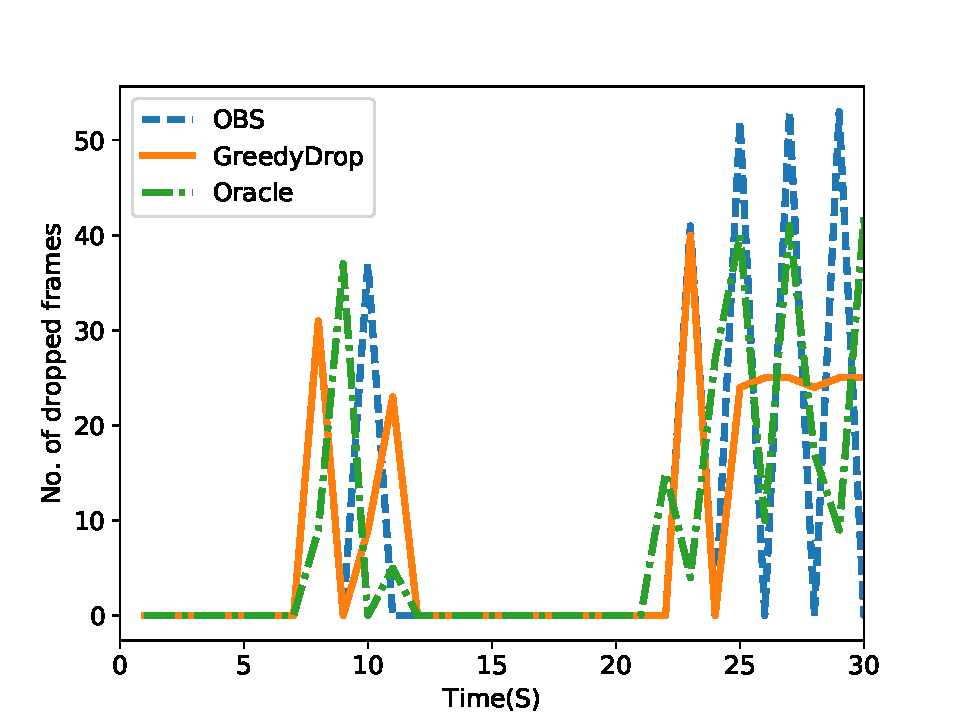
\includegraphics[width=\linewidth]{fig/drop-buffer.pdf}
\caption{No. of frame drop}
\label{fig:drop-buffer}\mylabel{fig:drop-buffer}
\end{subfigure}
\begin{subfigure}[b]{.45\columnwidth}
\centering
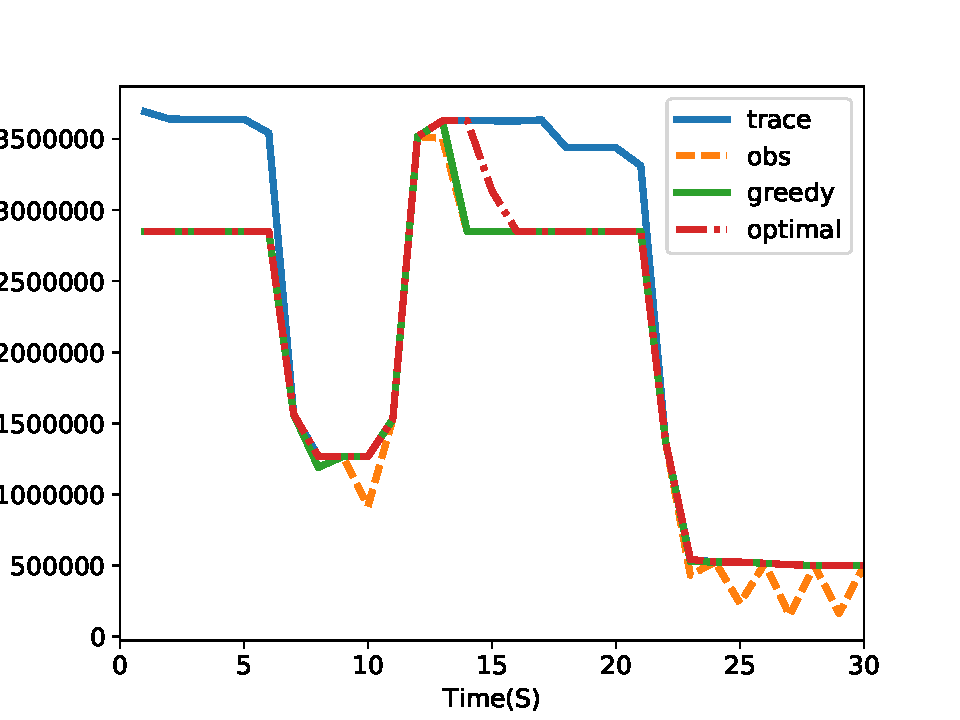
\includegraphics[width=\linewidth]{fig/drop-bandwidth.pdf}
\caption{Real-time throughput}
\label{fig:drop-bandwidth}\mylabel{fig:drop-bandwidth}
\end{subfigure}
\caption{Comparison of different frame drop strategy}
\vspace{-0.15in}
\end{figure} 
The reduction of frame drops is displayed in the table~\ref{tab_drop}. OBS dropped the most frames among three, and GreedyDrop reduce $15\%$, which is a prominent improvement. Morever the gap between GreedyDrop and Oracle is small, less than $5\%$. The frame drop and throughput is shown in Figures~\ref{fig:drop-buffer}~\ref{fig:drop-bandwidth}. The main period of frame dropping locates in 5-10s and 20-30s. All three algorithms perform similarly in 5-10s, but the Oracle will save more frames before the network recovers, and keep a high bandwidth at 10-15s. The frame drop of OBS waves at a high variance in 20-30s, but GreedyDrop almost keeps unchanged. Because GreedyDrop only drops the undecodable frames of the first GOP. For each GOP, the beginning is sent to receiver, and the rest ones is dropped, so for each time, the frame drops and the throughput keep still. Oracle also fluctuates, but with a small variance. Considering both time complexity and performance, GreedyDrop is a good choice.


\subsection{Greedy Adaptive Bitrate}
\begin{figure*}[htb]
\minipage{0.32\textwidth}
  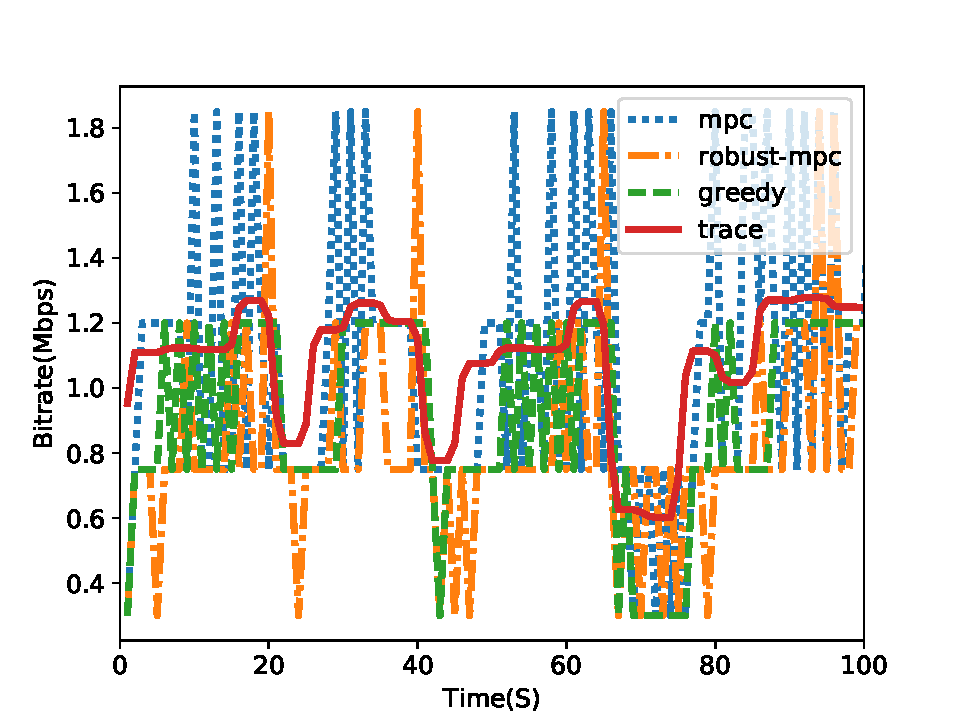
\includegraphics[width=\linewidth]{fig/specific_fcc.pdf}
  \caption{Throughput of FCC dataset}
  \vspace{-0.23in}
  \label{fig:fcc_specific}\mylabel{fig:fcc_specific}
\endminipage
\hfill
\minipage{0.32\textwidth}
  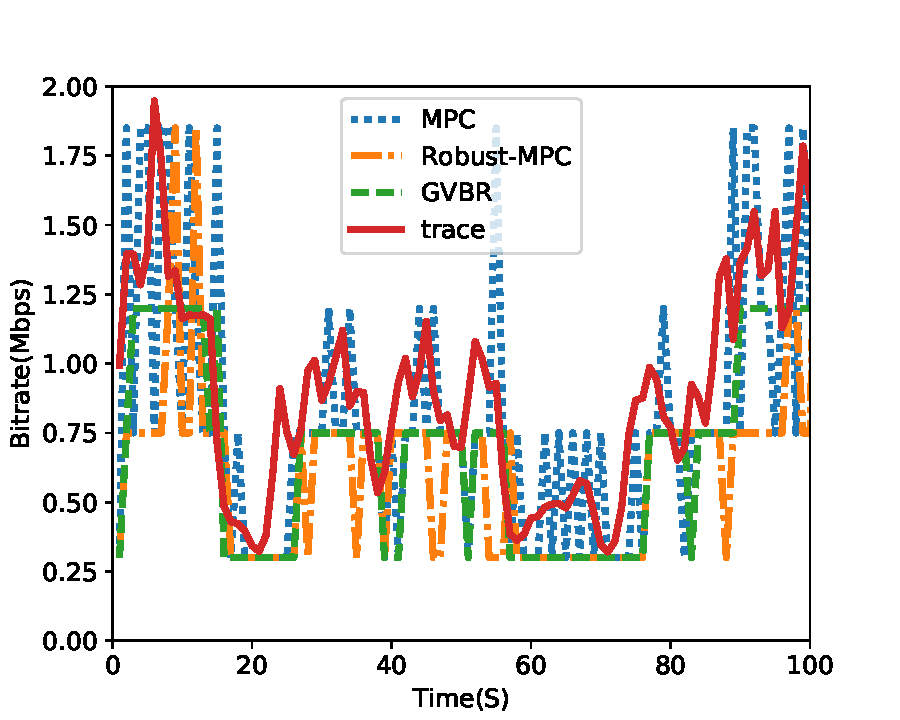
\includegraphics[width=\linewidth]{fig/specific_hsdpa.pdf}
  \caption{Throughput of HSDPA dataset}
  \vspace{-0.23in}
  \label{fig:specific_hsdpa}\mylabel{fig:specific_hsdpa}
\endminipage
\hfill
\minipage{0.32\textwidth}
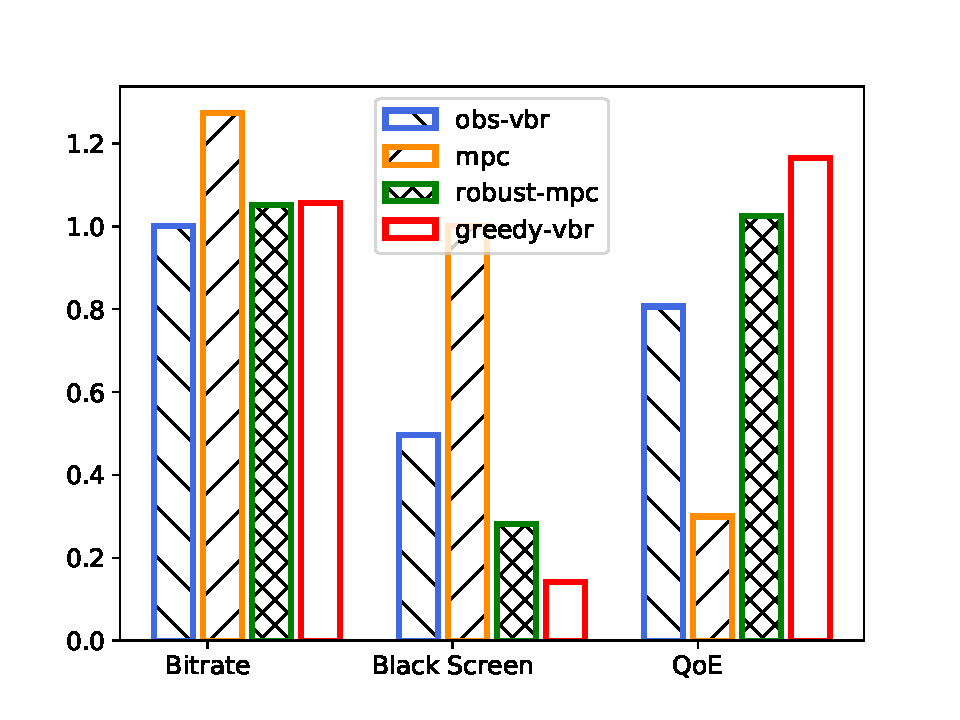
\includegraphics[width=\textwidth]{fig/massive_qoe.pdf}
\caption{Normalized bitrate, play failure and QoE}
\vspace{-0.23in}
\label{fig:vbr-qoe}\mylabel{fig:vbr-qoe}
\endminipage
\end{figure*}

\begin{figure*}[htb]
\minipage{0.32\textwidth}
  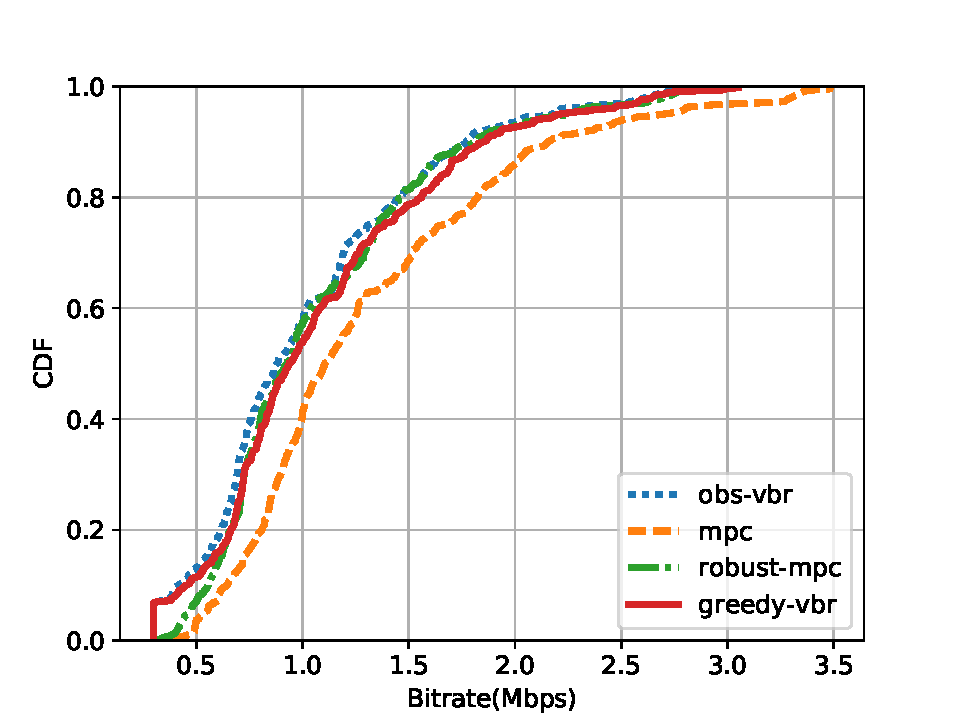
\includegraphics[width=\linewidth]{fig/massive-bitrate-cdf.pdf}
  \caption{CDF of Bitrate}
  \vspace{-0.25in}
  \label{fig:vbr-bitrate-cdf}\mylabel{fig:vbr-bitrate-cdf}
\endminipage
\minipage{0.32\textwidth}
  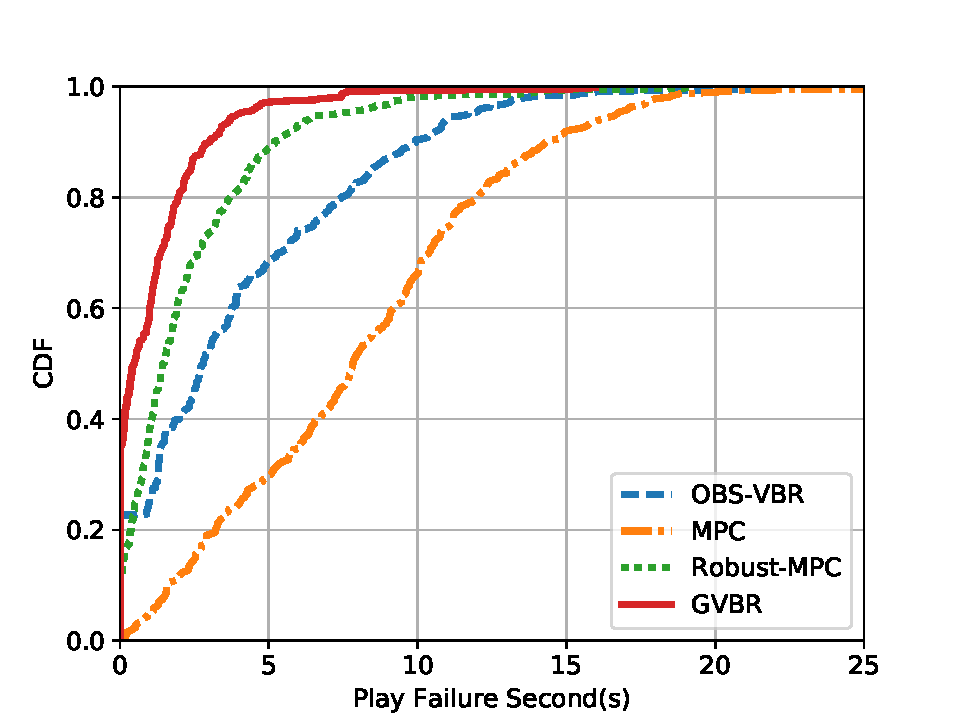
\includegraphics[width=\linewidth]{fig/massive-drop-cdf.pdf}
  \caption{CDF of Play Failure Seconds}
  \vspace{-0.25in}
  \label{fig:vbr-drop-cdf}\mylabel{fig:vbr-drop-cdf}
\endminipage
\minipage{0.32\textwidth}
  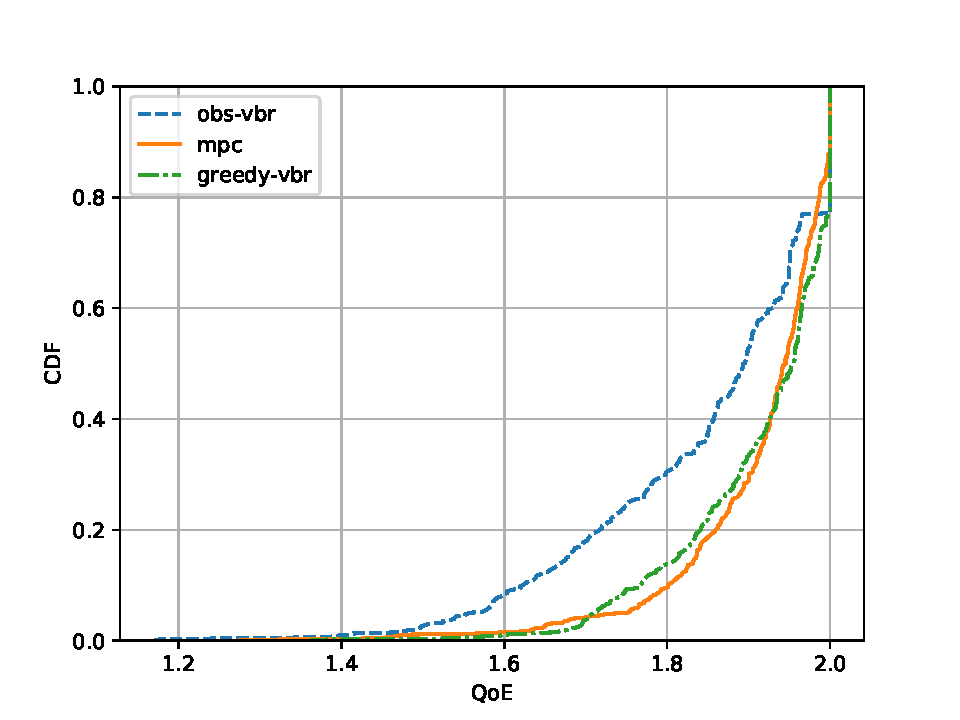
\includegraphics[width=\linewidth]{fig/massive-qoe-cdf.pdf}
  \caption{CDF of Normalized QoE }
  \vspace{-0.25in}
  \label{fig:vbr-qoe-cdf}\mylabel{fig:vbr-qoe-cdf}
\endminipage
\end{figure*} 
We compared GVBR algorihtm towards three algorithms which work excellently in VOD bitrate adaptation:
\begin{itemize}
  \item OBS-VBR: A simple but popular video adaptation method. Each time it chooses the bitrate exactly lower than the estimated bandwidth. In addition, use the default drop strategy in OBS. Harmonic mean is used for bandwidth estimation.
  \item MPC: use buffer state(number and size of frames, and type of frames, I/P/B) and bandwidth predictions to calculate the optimal bitrate operation in future several time slots. Use the first bitrate choice in next time slot.
  \item Robust-MPC: use the approach resembling MPC, but correct the estimated bandwidth by considering the prediction error in past several time slots. New estimated bandwidth equals the original estimated bandwidth divide the prediction error.
\end{itemize}
Robust-MPC is the state-of-art video adaptation algorithm. The MPC theory can also be applied to live streaming scenario.
Detailed comparison results are shown in Figures ~\ref{fig:fcc_specific} and \ref{fig:specific_hsdpa}. In these two figures, the real line is one real-world trace. Without predication error, MPC prefers to choose higher bitrate than Robust-MPC. Additionally, these two MPC algorihtm always fluctuate around the real bandwidth. In both cases, the MPC and Robust-MPC switch bitrate more frequently than GVBR. Because GVBR tends to choose the lower bitrate than the throughput, when the small bandwidth fluctuation happens, GVBR is less likely to shake. But MPC struggles to achieve the optimal utility, and when the bandwidth increases slightly, MPC has the potential to choose a higher bitrate to maximize the first item in \ref{vbr-formulation}.

A massive simulation is displayed in Figure \ref{fig:vbr-qoe}. We use the combined dataset, FCC and HSDPA to evaluate GVBR algorithm. Normalized QoE is calculated in the figure. Among all, MPC has the maximum bitrate QoE, because the bandwidth estimation is aggressive and MPC has the potential to choose higher bitrate. Three others reach almost the same average bitrate, with little difference, but GVBR is a little higher. With higher bitrate, MPC also drops the most frames, and the time of play failure is the longest. GVBR reduces the play failure to a small value, 50\% reduction compared with Robust-MPC. With higher bitrate and lower play failure, GVBR definitely preforms the best, with the highest QoE.

Cdf figures about bitrate, play failure and normalized QoE is as follows, Figure \ref{fig:vbr-bitrate-cdf}, \ref{fig:vbr-drop-cdf}, \ref{fig:vbr-qoe-cdf}. In \ref{fig:vbr-bitrate-cdf}, GVBR lies in the right of Robust-MPC and OBS, with a higher bitrate. $98\%$ of the paly failure is less than 5s in GVBR, about 40\% play fluently with no failure. Only 2\% of GVBR receives poor QoE, the rest 98\% has a high QoE falling in [0.8,1].

The total frame drops compared with original OBS are reduced by 96\%. The play failure time of original OBS method with constant bitrate is 26s in average, and GVBR has a one-second play failure time.

As all, GVBR achieves a higher bitrate, and at the same time reduces the play failure significantly.

